% ------------------------------------------------------------------
%  Supplementary Information for the AETIA manuscript.
%  Build: latexmk -pdf Supplementary.tex  (or `make`)
% ------------------------------------------------------------------
\documentclass[11pt,a4paper]{article}
\usepackage[utf8]{inputenc}
\usepackage[T1]{fontenc}
\usepackage{lmodern}
\usepackage[margin=2.5cm]{geometry}
\usepackage{setspace}
\usepackage{graphicx}
\usepackage{amsmath}
\usepackage{booktabs}
\usepackage{longtable}
\usepackage{array}
\usepackage{xspace}
\usepackage{xcolor}
\usepackage[super,sort&compress,numbers]{natbib}
\usepackage[hidelinks]{hyperref}
\usepackage{url}
\graphicspath{{figures/supp/}}
\bibliographystyle{naturemag}
\setcitestyle{super,open={},close={}}

\newcommand{\toolname}{AETIA\xspace}
\newcommand{\toolexpansion}{Agentic Evidence Tracing of Infectious Aetiology\xspace}
\newcommand{\mngs}{mNGS\xspace}
\newcommand{\filmarray}{FilmArray\xspace}
\newcommand{\rfive}{R5\xspace}
\newcommand{\vtwenty}{v20\xspace}
\newcommand{\kmuh}{KMUH\xspace}
\newcommand{\tvgh}{TVGH\xspace}
\newcommand{\tsgh}{TSGH\xspace}
\newcommand{\todo}[1]{\textcolor{red}{[#1]}}
\renewcommand{\thefigure}{S\arabic{figure}}
\renewcommand{\thetable}{S\arabic{table}}

\title{Supplementary Information\\[4pt]\large Auditable multimodal integration of metagenomic sequencing and clinical evidence identifies causative pathogens in lower respiratory tract infection}
\author{}
\date{}

\begin{document}
\sloppy
\onehalfspacing
\maketitle
\tableofcontents

\clearpage
\section*{Supplementary Figures}
\addcontentsline{toc}{section}{Supplementary Figures}

\begin{figure}[h]
  \centering
  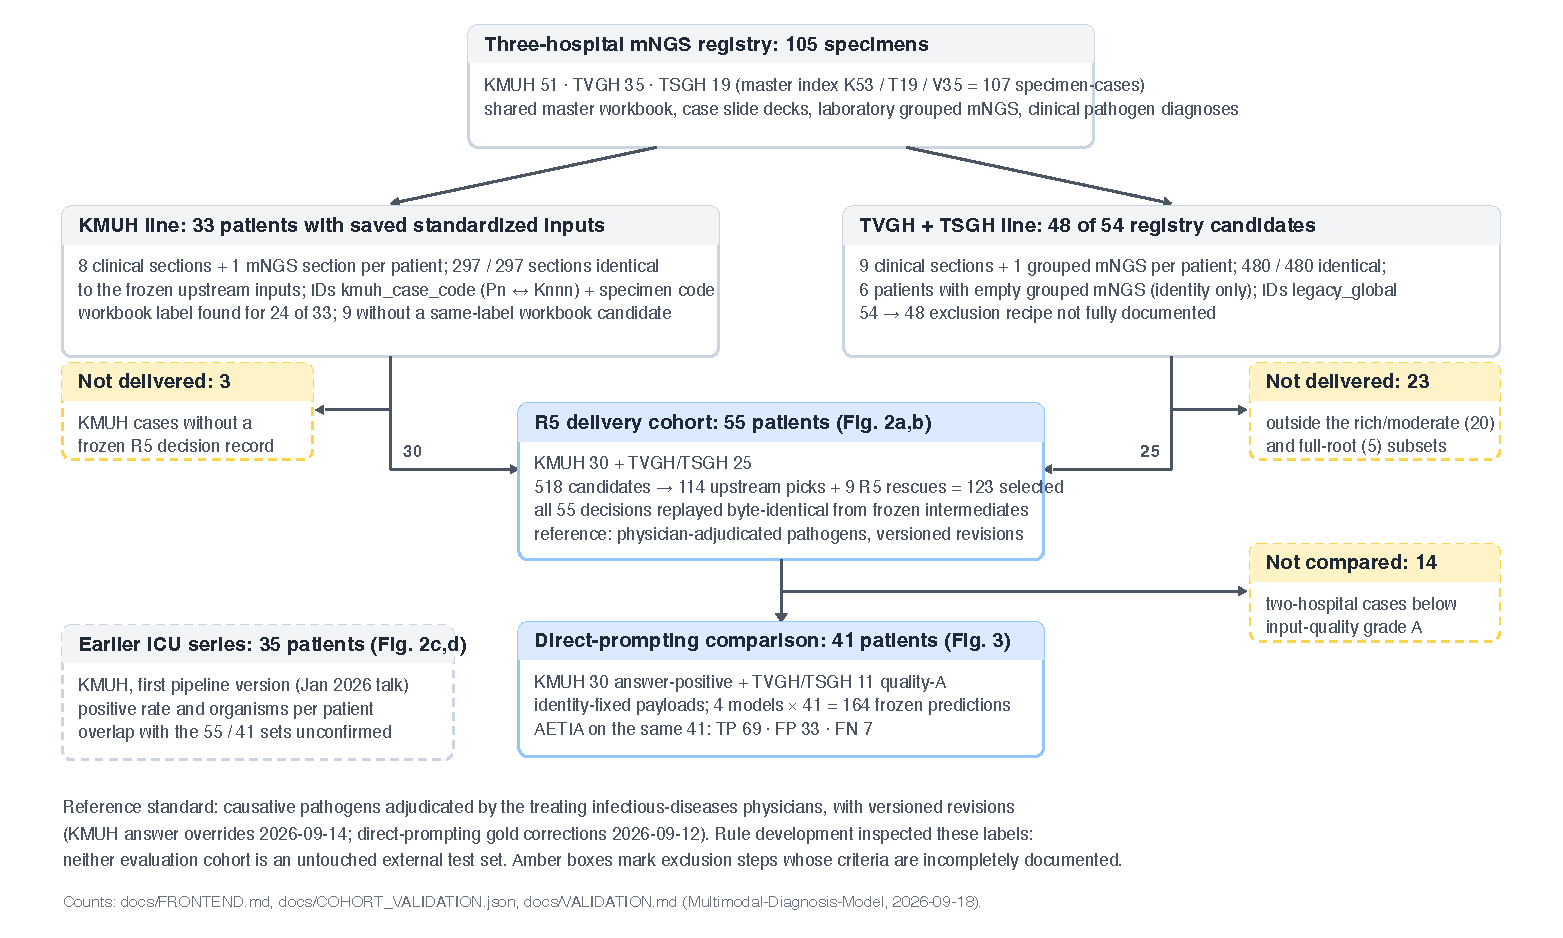
\includegraphics[width=\textwidth]{figS1_cohort_flow}
  \caption{\textbf{Cohort flow.} From the three-hospital \mngs registry (105 specimens; Table~1) through the two hospital lines to the \rfive delivery cohort ($n=\todo{55}$) and the direct-prompting comparison cohort ($n=\todo{41}$). Amber boxes, exclusion steps whose criteria are incompletely documented in the source materials; dashed grey box, the earlier 35-patient intensive-care series (main Fig.~2c,d), whose overlap with the evaluation cohorts is \todo{unconfirmed}. Counts from the repository's cohort validation of 2026-09-18.}
  \label{fig:s1}
\end{figure}

\clearpage
\section*{Supplementary Tables}
\addcontentsline{toc}{section}{Supplementary Tables}

\begin{table}[h]
\centering
\caption{\textbf{\mngs organism features computed before scoring.} Source: \texttt{upstream/tools/rank\_mngs\_candidate\_microbes.py}, \texttt{upstream/tools/mngs\_common.py}, \texttt{deterministic\_mngs\_max\_scorer.py} (\texttt{dominance\_by\_record}).}
\label{tab:s1}
\footnotesize
\begin{tabular}{p{2.8cm}p{2.4cm}p{9.4cm}}
\toprule
Feature & Values & Definition \\
\midrule
Control-subtracted priority & 1--5 & 1: NTC$=$00 and RK00; 2: RK8 and NTC$=$00; 3: RK00; 4: RK8; 5: NTC$=$00 only. Code score 1.0, 0.85, 0.65, 0.45, 0.30. \\
Read percentile & 0--1 & Percentile of $\log_{10}(\text{reads}+1)$ among all organisms in the run. \\
Final score / label & high, medium, low & $0.6\times$code score $+\,0.4\times$percentile; high $\ge 0.70$, medium $\ge 0.45$. \\
Read tier & R0--R4 & R0: 1--9 reads; R1: $\ge 10$; R2: $\ge 100$; R3: $\ge 1{,}000$; R4: $\ge 10{,}000$. \\
Dominance tier & D0--D3 & Per specimen record; top organism: D3 if reads $\ge 10\times$ runner-up, D2 if $\ge 3\times$, else D1; every other organism D0. \\
Specimen alignment & aligned, sterile/systemic, non-aligned & From the \mngs-to-specimen assignment and the target site (lower respiratory tract). \\
Hospital support & per module & Same-organism support from culture, \filmarray/galactomannan, molecular microbiology; ``Support'', ``Not support'' or ``Unknown''. \\
Host context & V0--V3, O0--O2 & Host-vulnerability tier and opportunistic-coverage level; host expansion when V2--V3 or O1--O2. \\
\bottomrule
\end{tabular}
\end{table}

\begin{table}[h]
\centering
\caption{\textbf{Signal tiers and causative levels of the deterministic scorer (\vtwenty).} Source: \texttt{deterministic\_mngs\_max\_scorer.py}, functions \texttt{m1\_strong}, \texttt{m2\_moderate}, \texttt{m3\_protected}, \texttt{m4\_weak}, \texttt{set\_candidate\_level\_from\_tier}, \texttt{level3\_pickable}, \texttt{pickable}. Conditions are evaluated in order; the first satisfied tier applies.}
\label{tab:s2}
\footnotesize
\begin{tabular}{p{2.2cm}p{12.9cm}}
\toprule
Tier / level & Condition \\
\midrule
M1 strong & priority 1--2 and R3--R4; or priority 1--2 and percentile $\ge 0.85$; or D3 and $\ge$R2 and priority $\le 3$. \\
M2 moderate & priority 1--2 and R2 and percentile $\ge 0.75$; or D2--D3 and $\ge$R2 and priority $\le 3$; or same-organism auxiliary support and $\ge$R1 and priority $\le 3$; or protected pathogen (not reactivation virus or mould), $\ge$R1, priority $\le 3$, label not low; or R3--R4 and priority $\le 4$ and label not low; or \textit{P.~jirovecii} with R1--R2 and priority $\le 3$; or Mucorales at priority 1 with percentile $\ge 0.60$. Reactivation viruses and \textit{Aspergillus} use dedicated clauses. \\
M3 protected & retention condition of a protected pathogen; or priority 1--2 with R0--R2; or priority $\le 3$ with percentile $\ge 0.60$ above R0; or priority $\le 3$ with high/medium label and R1--R2; or priority 3 with R1--R2 and non-host auxiliary support; or priority 4 with R4. \\
M4 weak & priority 4--5; or label low; or R0--R1; or non-aligned specimen. \\
M5 background & organism on the background list. \\
\midrule
Level 1 & M1, aligned or sterile specimen, and (D3 or R3--R4). \\
Level 2 & other M1; M2 with aligned or sterile specimen. \\
Level 3 & M2 non-aligned; M3; M4 under host expansion when plausible (not reactivation virus, colonizer or non-aligned; with non-host support, protected status, or priority $\le 3$ with R1 and high/medium label). \\
Level 4 & other M4; any organism demoted by a guardrail. \\
Level 5 & M5. \\
\midrule
Picked & level 1--2; level 3 with protected status, an oral-flora/respiratory-commensal representative rule, related typical-pneumonia context, direct support from culture, \filmarray/galactomannan or molecular testing, or (host expansion) priority $\le 2$ with $\ge$R2 or D2--D3; \textit{Candida}/generic yeast never at level 3 without invasive support. Fallback: level-4 ``best available'' when nothing is pickable. \\
\bottomrule
\end{tabular}
\end{table}

\begin{table}[h]
\centering
\caption{\textbf{Guardrail rule identifiers of the deterministic scorer.} All 33 \texttt{R-S4-*} identifiers found in \texttt{deterministic\_mngs\_max\_scorer.py}. Descriptions paraphrase the identifier and the rule body; \todo{verify each against the code before submission}.}
\label{tab:s3}
\footnotesize
\begin{tabular}{p{7.0cm}p{8.0cm}}
\toprule
Identifier (\texttt{R-S4-\ldots}) & Effect \\
\midrule
BACKGROUND & background organism, level 5 \\
CANDIDA-BLOOD-STERILE-CONTEXT & \textit{Candida} retained on blood/sterile-site evidence \\
CANDIDA-HOSPITAL-NONINVASIVE-NOT-PICKED & \textit{Candida} with only non-invasive hospital support not picked \\
CANDIDA-RESP-CONTEXT-NOT-PICKED & respiratory \textit{Candida} context not picked \\
CANDIDA-RESP-L3 & respiratory \textit{Candida} held at level 3; picked only with invasive support \\
COMMON-HOSPITAL-R0R1-NONDOMINANT-PICKED-OMIT & common hospital organism with R0--R1, non-dominant: omitted from picks \\
GENERIC-UNIDENTIFIED-HOSPITAL-LABEL & generic labels (e.g. ``Gram-negative bacilli'') never picked \\
HERPES-HOST-R2R3-NONDOMINANT-REVIEW & herpesvirus with host-only support, R2--R3, non-dominant: review only \\
HERPES-R4-NONDOMINANT-HOST-ONLY-REVIEW & herpesvirus with R4 but non-dominant and host-only: review only \\
IMPOSSIBLE-INFECTION-SOURCE & organism cannot be a pulmonary infection source \\
L3-MNGS-ONLY-HOST-LOW-NONDOMINANT & level-3 \mngs-only organism with low, non-dominant reads not picked \\
LOW-ACTIONABILITY-VIRUS-PICKED-OMIT & EBV, HHV-6/7 and similar omitted from picks \\
LOW-PULM-SPECIFICITY-ATYPICAL-L4 & atypical organism of low pulmonary specificity, level 4 \\
LOW-PULM-SPECIFICITY-ENV-L4 & environmental organism of low pulmonary specificity, level 4 \\
LOW-SPECIFICITY-VIRUS-L4 & low-specificity virus, level 4 \\
MNGS-ONLY-NONDOMINANT-NON-TYPICAL-PICKED-OMIT & \mngs-only, non-dominant, non-typical pneumonia organism omitted \\
MNGS-R0R1-HOST-ONLY-NONPROTECTED-PICKED-OMIT & R0--R1 with host-only support, non-protected: omitted \\
NON-CORE-RESP-VIRUS-PICKED-OMIT & non-core respiratory virus omitted from picks \\
NONPULMONARY-CULTURE-CONTEXT-ONLY & culture at a non-pulmonary site is context only \\
ORAL-ASPIRATION-FLORA-L3 & oral/aspiration flora representative retained at level 3 \\
ORAL-ASPIRATION-FLORA-MNGS-ONLY-NONDOMINANT-L4 & \mngs-only, non-dominant oral flora, level 4 \\
RARE-YEAST-HOSPITAL-MNGS-L3 & rare opportunistic yeast with hospital and \mngs support, level 3 \\
RARE-YEAST-MNGS-ONLY-CONTEXT & rare yeast with \mngs only: context \\
RELATED-REPRESENTATIVE-HOSPITAL-CONTEXT & related-organism hospital context supports a representative \\
RESP-COMMENSAL-L3 & respiratory commensal retained at level 3 \\
RESP-COMMENSAL-L4 & respiratory commensal, level 4 \\
SAME-REPRESENTATIVE-GROUP-PICKED-OMIT & one representative per taxonomic group; others omitted \\
SKIN-ENV-YEAST-L4 & skin/environmental yeast, level 4 \\
SKIN-LOW-SPECIFICITY-BACTERIA-L4 & skin flora of low specificity, level 4 \\
TRACE-PROTECTED-WATCHLIST-PREFERRED & trace-read protected pathogen kept on a watch-list, not picked \\
WATER-ENV-GNB-L4 & water-borne environmental Gram-negative, level 4 \\
WATER-ENV-LOW-SPECIFICITY-PICKED-OMIT & water-borne organism of low specificity omitted from picks \\
WEAK-MOLD-HOST-ONLY-PICKED-OMIT & weak mould signal with host-only support omitted \\
\bottomrule
\end{tabular}
\end{table}

\begin{table}[h]
\centering
\caption{\textbf{Evidence-module thresholds used by \rfive.} Sources: \texttt{RAG\_re/config/default.json}, \texttt{RAG\_re/config/formal\_merge\_full\_a.json}, \texttt{RAG\_re\_casefit/config/default.json}, \texttt{RAG\_re\_clinical/config/clinical\_v1.json}, \texttt{OBER\_patient\_delivery/generate\_r5\_final\_decisions.py}.}
\label{tab:s4}
\footnotesize
\begin{tabular}{p{2.0cm}p{13.0cm}}
\toprule
Module & Setting \\
\midrule
A retrieval & PubMed E-utilities; query \texttt{"organism"[Title/Abstract]} AND (site terms in title/abstract); publication cutoff 2026-06-30; at most 10 articles; 0.34 s between requests; literature also retrieved for upstream picks (\texttt{literature\_on\_baseline\_picked = true}). \\
A judgement & support requires exact species, human clinical evidence, target-site match and a valid evidence span ($\le 20$ contiguous words); positive when $\ge 3$ valid supports among $\ge 5$ judgeable articles; otherwise abstain. \\
A1 case-fit & per-article verdict strong / partial / mismatch / insufficient (Methods); aggregation thresholds in config: $\ge 2$ strong for high, $\ge 1$ strong or $\ge 3$ partial for moderate, $\ge 5$ judgeable articles. \rfive uses strong $\ge 2$ or strong$+$partial $\ge 7$. \\
B & absolute axis: M1/M2 or R3/R4; relative axis: dominance $\ge$ D2, or priority $\le 1$ with percentile $\ge 0.8$; site alignment required; NTC ratio and RPM gates not required (\texttt{require\_ntc\_ratio = false}, \texttt{require\_rpm = false}). \\
C & positive modules: culture, \filmarray, \filmarray/galactomannan, targeted molecular, molecular microbiology, PCR, antigen, galactomannan; grades C3 / C2 / C1 / C0 / CNEG as in Methods; respiratory \textit{Candida} with culture only $\rightarrow$ C1. \\
D & pass / guarded / block / unknown; reported, not gated. \\
Temporal & window 3 days before and after the anchor (research arms only). \\
\rfive & \texttt{picked OR C3 OR ((A1\_strong >= 2 OR A1\_match >= 7)} \texttt{AND site\_aligned AND (B\_absolute OR B\_relative))}; rule id \texttt{R5\_A1\_UNION\_AND\_B\_LOOSE}. \\
\bottomrule
\end{tabular}
\end{table}

\begin{table}[h]
\centering
\caption{\textbf{Language models, prompts and configurations by stage.} SHA-256 prefixes of the files in the code repository at the time of writing (2026-09-20). \todo{Confirm the model identifiers and reasoning settings used for the reported runs from the run manifests; confirm the formatter and vision models.}}
\label{tab:s5}
\footnotesize
\begin{tabular}{p{3.0cm}p{3.2cm}p{5.2cm}p{2.8cm}}
\toprule
Stage & Model / setting & File & SHA-256 (prefix) \\
\midrule
Formatter (raw $\rightarrow$ standardized JSON) & \todo{model} & \path{upstream/core/llm_parser.py} & -- \\
Host/laboratory agent & \todo{GPT-5} & \path{agents/prompts/CBC_Lab_underlying_prompt.txt} & \texttt{0929360cfb5d} \\
Culture agent & \todo{GPT-5} & \path{agents/prompts/culture_agent_prompt.txt} & \texttt{e1631735b119} \\
\filmarray and GM agent & \todo{GPT-5} & \path{agents/prompts/filmarray_GMtest_prompt.txt} & \texttt{2a092516ff13} \\
Imaging agent & \todo{GPT-5} & \path{agents/prompts/image_agent_prompt.txt} & \texttt{b0ea51281d8f} \\
Molecular agent & \todo{GPT-5} & \path{agents/prompts/molecular_microbiology_prompt.txt} & \texttt{802ccf52ac71} \\
\mngs-to-specimen & \todo{GPT-5 or deterministic v4} & \path{agents/prompts/mNGS_to_specimen_prompt.txt} & \texttt{643dcf157308} \\
Deterministic summary & rules v4 & \path{tools/build_deterministic_summary.py} & -- \\
Scorer & rules v19 (reported) / \vtwenty (current) & \path{tools/deterministic_mngs_max_scorer.py} & -- \\
Missed-candidate review & \todo{GPT-5} & prompt in \path{tools/review_missed_mngs_candidates.py} & -- \\
Article judge (A) & GPT-5.6 Luna, reasoning low, 1,200 tokens & \path{RAG_re/prompts/article_support_v1.txt}; \path{config/default.json}; \path{formal_merge_full_a.json} & \texttt{af4178902c50}; \texttt{bc123c20c743}; \texttt{b3ca56742dce} \\
Case-fit (A1) & GPT-5.6 Luna, reasoning low, 1,400 tokens & \path{RAG_re_casefit/prompts/article_casefit_v1.txt}; \path{evidence_span_repair_v1.txt}; \path{config/default.json} & \texttt{e495aef60640}; \texttt{f6f15feca9d9}; \texttt{a9f387850b01} \\
Clinical rules (B, C, D) & \texttt{clinical\_v1} & \path{RAG_re_clinical/config/clinical_v1.json} & \texttt{41121351788c} \\
\rfive & rule \path{R5_A1_UNION_AND_B_LOOSE} & \path{OBER_patient_delivery/generate_r5_final_decisions.py} & -- \\
Rationale & GPT-5.6 Luna, reasoning low & \path{generate_llm_rationales.py} & -- \\
Direct prompting & gpt-5.6-sol/luna/terra, gpt-6-astra; reasoning medium; 4,000 tokens & \path{LLM_test/direct_raw_benchmark/prompt_v1.txt} & \texttt{961087b8acdf} \\
\bottomrule
\end{tabular}
\end{table}

\clearpage
\section*{Supplementary Notes}
\addcontentsline{toc}{section}{Supplementary Notes}

\subsection*{Supplementary Note 1. Missed-candidate safety-review prompt}
The review prompt is embedded in \texttt{upstream/tools/review\_missed\_mngs\_candidates.py} (\texttt{build\_prompt}). Its operative content, paraphrased: the model is a safety reviewer for suspected pulmonary infection and may not replace the deterministic picks; it receives the review queue with rank, reads, tiers, dominance, level and guardrail reasons, the deterministic output, the hospital-side summary and the \mngs-to-specimen classes; it returns four categories (\texttt{review\_high\_priority}, \texttt{review\_context\_needed}, \texttt{review\_low\_specificity}, \texttt{omitted\_with\_reason}); it must not upgrade for immunocompromise or protected status alone; respiratory \textit{Candida} and generic yeast evidence is low-specificity unless same-species invasive evidence exists; different \textit{Candida} species are never aliases; CMV, HSV and VZV are flagged as reactivation unless primary pulmonary disease is supported and EBV is never a pulmonary candidate; very high herpesvirus reads with a non-dominant pattern and host-only support remain context-needed; oral and aspiration flora are grouped into strict anaerobes, broad commensals and atypical oral organisms with tier rules for each; water-borne Gram-negatives, GI-only pathogens and coagulase-negative staphylococci or corynebacteria have explicit demotion rules; and the output is a JSON object with Traditional-Chinese rationale fields. \todo{Reproduce the prompt verbatim (with permission) or provide it as Supplementary Data.}

\subsection*{Supplementary Note 2. Direct-prompting baseline prompt}
File \texttt{LLM\_test/direct\_raw\_benchmark/prompt\_v1.txt} (SHA-256 prefix \texttt{961087b8acdf}), original in Traditional Chinese. English rendering:

\begin{quote}\small
You are an infectious-diseases clinical reviewer. Using only the single patient's data provided here, decide which microorganisms are most likely the clinical causative pathogens of the current pulmonary or lower-respiratory-tract infection episode.

This is the Direct-Raw baseline: do not use external search, PubMed, RAG, AETIA, any candidate pool or any earlier model result. The raw \mngs list may contain contamination, colonization, background organisms, low-level detections and organisms unrelated to the site of infection; ``detected'' does not mean ``pathogen''. Judge from the \mngs reads and RK/NTC codes, the specimen site, cultures, molecular tests, imaging, host status and timing. Respiratory \textit{Candida}, low-specificity environmental organisms, skin flora and latent or reactivated viruses must not be listed as the infection source merely because they were detected. A positive result from a non-pulmonary specimen must not be treated as a pulmonary source without a pulmonary link. An empty array means ``no record available'', not a negative test. You may select zero, one or several pathogens; do not force an answer. Put only the organisms you finally judge to be the infection source in \texttt{predicted\_pathogens}; if evidence is insufficient, put them in \texttt{excluded\_detected\_organisms} or \texttt{limitations}. Name pathogens at species level; do not merge different \textit{Candida} or other species. Output must follow the given JSON schema; supporting evidence, counter-evidence, reason and limitations should be short and auditable, and hidden reasoning must not be output.
\end{quote}

\subsection*{Supplementary Note 3. Case examples}
\todo{Two anonymized cases from the January 2026 series (main text, Results): (1) \textit{Klebsiella pneumoniae} selected with 68,569 \mngs reads, bilateral consolidation with pleural effusions, rising CRP and worsening hypoxaemia, with \textit{Candida albicans} excluded as colonization; (2) \textit{Candida tropicalis} selected on multiple positive blood-culture sets and high BALF reads (C3 direct path). Replace with the delivered \rfive records: selected organisms, rule paths, module results (A/A1 counts with PMIDs, B axes, C grade, D state), the audited rationale, and the reference labels. Obtain approval for case-level presentation.}

\subsection*{Supplementary Note 4. Version boundaries and replay}
The \todo{55} reported \rfive decisions were generated from upstream outputs scored with rule version v19 (\texttt{mngs\_deterministic\_level\_only\_v19\_low\_specificity\_taxonomy}). The v19 scorer was recovered and verified to reproduce all \todo{55} saved scorer outputs from the saved summaries and ranked \mngs. The current scorer \vtwenty (\texttt{mngs\_deterministic\_level\_only\_v20\_central\_taxonomy\_profile}) moves the taxonomy profiles to a central module and removes a retired language-model scoring branch; replayed on the same inputs it reproduces the picked set of all \todo{55} patients and the candidate names in all \todo{55}, changes candidate levels in \todo{15} patients (\todo{15} shared-candidate level changes in total) and the pick order alone in \todo{5}, and reproduces the merge-stage picked sets and review-tier membership in all \todo{55}. The clinical-summary replay used the current patient directories rather than a proven frozen agent snapshot; three patients differ in in-hospital evidence between the reconstructed and the saved summaries. None of these differences alters the reported selections. Source: \texttt{docs/UPSTREAM\_REPLAY\_SUMMARY.json}, \texttt{docs/UPSTREAM\_RECOVERY.md}, \texttt{docs/VERSIONS.md}.

\subsection*{Supplementary Note 5. Evaluation outputs to be added}
\todo{Per-patient tables for the 55- and 41-patient cohorts (predicted and reference sets per method; TP/FP/FN); per-hospital metrics; macro metrics, any-hit, all-hit and exact-set-match rates; the list of the 9 rescued organisms with rule paths and correctness; error analysis of false negatives (absent from report, below tier, guardrail, review tier not carried) and false positives (upstream pick versus rescue); confidence intervals.}

% no citations in the Supplementary at present; add \bibliography{references} when needed
\end{document}
